\section{Extras}

\prtodoi{This is where I am putting text/figures that don't fit in main text, worth checking every so often to maybe re-incorporate}

\subsection{Leaderboard Perturbations}
\prtodo{This section isn't well fleshed out, unclear if there is even enough room for it}

Thus far, we have limited our methodology to only using real leaderboard data and excluded artificial modifications or synthetic data.
However, the \irt{} leaderboard model opens the possibility to principled perturbations of the generative story to observe the causal effect on leaderboard efficacy.
For example, we can modify the generative story to incorporate phenomena like annotation error rates---a problem in most crowdsourced datasets.
Although errors can take many forms, we test one simple case where the annotator's error causes all agents to answer incorrectly (e.g., an ill-posed question or incorrect answer annotation).
While perturbations could be more sophisticated, we use this simple one to quantify a known phenomena in crowdsourced data.


\subsection{Effects of Leaderboard Perturbations}

The final set of experiments to motivate \irt{} for evaluation consider the effects of perturbations that reproduce effects like annotation error.
For this work, we focus on annotation errors which cause all models to be given a score of zero for erroneous items.
Of note, is that these types of questions are indistinguishable from examples that are too difficult for current models so with current techniques that select ``hard'' subsets would not help distinguish better models from worse models.
We expect that these errors should increase the perceived statistical strength of traditional tests due to increased sample size, having no effect on the \abr{see}, and should adversely affect ranking stability.
These results will be connected back to real data by sampling examples that all models are incorrect on and manually estimating the prevalence of this type of error which can in turn be used to estimate its effect on the \squad{} evaluation.

Combined, our preliminary and proposed experiments are intended to show that current evaluation methodologies are inadequate and that \irt{} influenced evaluations can mitigate some of their problems.
Next, we discuss another way that \irt{} can be useful in leaderboards.

\prtodoi{Experiments currently don't involve theoretical/simulated data, although this might make the paper stronger. Perhaps appendix material?}


\subsection{Stability (old)}
\begin{figure}[t]
    \centering
    \subcaptionbox{
        Error rate by accuracy of better model versus the sample size.
        \label{fig:stability-max}
    }{
        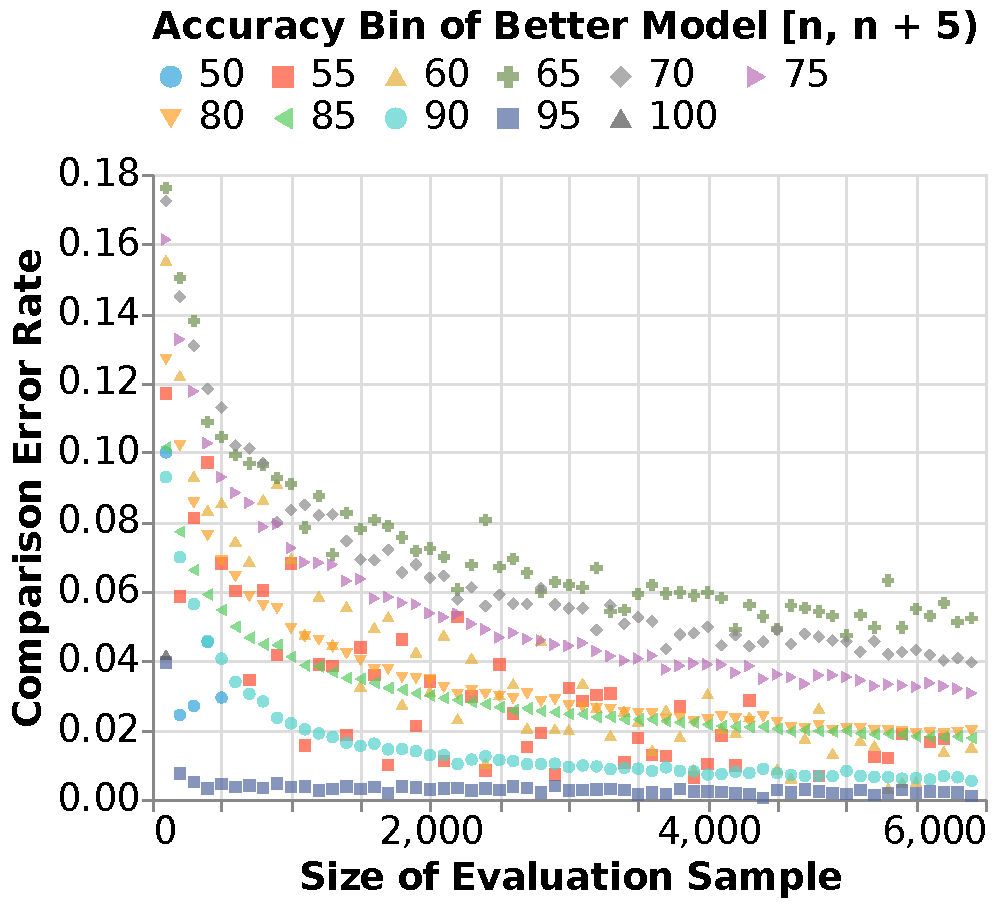
\includegraphics[width=.45\textwidth]{error_by_max_score.pdf}
    }
    \hspace{.01\textwidth}
    \subcaptionbox{
        Error rate by accuracy difference versus the sample size.
        \label{fig:stability-diff}
    }{
        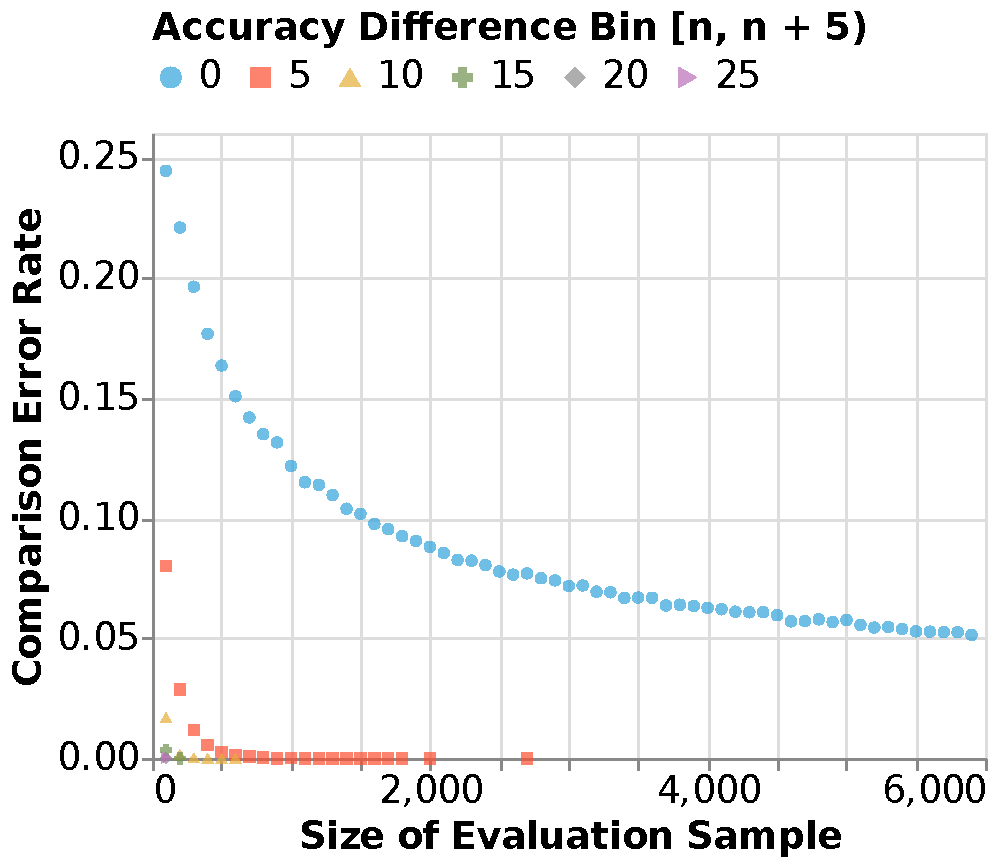
\includegraphics[width=.45\textwidth]{error_by_diff.pdf}
    }
    \caption{
        The comparison error rate from ranking stability experiments as a function of the maximal score between two agents and the difference between scores.
        Most errors occur between 65\% and 80\% accuracy and when differences are less than five percentage points.
    }
    \label{fig:stability-old}
\end{figure}

\subsection{A Comparison of Statistical Tests}

Based on the idea from \irt{} that maximally informative items---those that models have fifty percent chance of answering correctly---improve statistical testing we compare \irt{} statistical significance (Section~\ref{ch:isicle:reliable}) to that of several common tests.
Figure~\ref{fig:compare-test} compares the \irt{} test to the McNemar test, Student-T test, Standard Error of Mean, and the Wilcoxon test.
The McNemar, Student-T, and Wilcoxon tests behave similarly and have higher rates of agreement compared to the other two tests (Figure~\ref{fig:test-agree}); Figure~\ref{fig:irt-dist} shows the distribution of P-Values when tests disagree.
\prtodoi{Write Takeaway/summary}

\begin{figure*}[t]
    \centering
    \includegraphics[width=\textwidth]{compare_tests}
    \caption{
        TODO
    }
    \label{fig:compare-test}
\end{figure*}

\begin{figure}[t]
    \centering
    \includegraphics[width=\columnwidth]{test_agreement}
    \caption{
        TODO
    }
    \label{fig:test-agree}
\end{figure}

\begin{figure}[t]
    \centering
    \includegraphics[width=\columnwidth]{disagree_pvalues}
    \caption{
        TODO
    }
    \label{fig:disagree-dist}
\end{figure}



\subsection{Residual Analysis}

\prtodoi{Calculate residual analysis and include here
    residuals as is common in psychometrics~\citep{haberman2009residuals,sinharay2014fit}.
    TODO: look into this residual fit method~\citep{sinharay2014fit}.
}
\prtodoi{START COMMENTED TEXT}
Fundamentally, there are two kinds of evaluations that require different type of test data: Cranfield paradigm evaluations that approximate user satisfaction and evaluations testing specific skills.

In these tests, examples are not randomly drawn from a distribution, but instead hand-picked.
In contrast, Cranfield paradigm evaluations are ultimately testing if a user would be satisfied with a model's responses.
Satisfaction is approximated by randomly drawing users whose source distribution is assumed to be similar to the true user distribution, assuming that those users ask similar questions, and assuming that their satisfactions with model answers are positively correlated.
Information retrieval and question answering evaluations extended this paradigm by creating automated rules for deciding whether a model's response is equivalent to the annotated answer and thus would satisfy a real user(e.g., \squad{}'s F1 text overlap measure).
In diagnostic tests, all the examples matter since they are directly linked to establishing whether models demonstrate specific skills, but in statistical satisfaction evaluations examples are not individually important.
On the contrary, we argue that comparatively few examples matter in determining the ranking of models and propose that these examples can be identified with a latent variable model.
\prtodoi{END COMMENTED TEXT}

\prtodoi{START COMMENTED TEXT}
This is from viz section, some of it could work here if there is space
Similarly to Manifold~\citep{zhang2019manifold}, the goal of the model-centric view is to understand the differences---based on predictions---between models.
Another approach to a model-centric views instead attempts at characterizing the performance along partitions of the data~\citep{liu2018answer}.
For example, \citet{arendt2020crosscheck} propose faceted histograms as a way to ``un-aggregate'' metrics to inspect \qa{} accuracy by factors like question type and confidence.
In addition to visualizing which instances pairs of models agree as in Manifold, we propose integrating \irt{} parameters to better identify instances that have a larger influence over the output ranking.

A dominant approach to inspecting models examines their performance on individual examples or partitions of examples sharing a trait~\citep{wadhwa2018compare}.
In addition to domain-relevant traits, we can guide example sample selection with \irt{} which makes it more likely to identify important issues over random sampling~\citep{wadhwa2018compare} while still combining careful specification of error types~\citep{wu2019errudite}.
Similarly, visualizations can use the multidimensional \irt{} parameters for clustering which can also be combined with domain-specific attributes like question type or topic.
\prtodoi{END CoMMENTED TEXT}

\prtodoi{
    PR: maybe re-incorporate somewhere
    tradoff stat power and type 1 error
    At least for McNemar test, statistical power increases with agreement rate, which increases when p(correct) approaches 1.
    The tradeoff though is Type 1 error. This section could discuss this tradeoff as is discussed and plotted in~\ref{ch:isicle:apx:mcnemar}
    Discuss how we should look at type 1 error and power, and tradeoff.
    type 1 error and power are used in psychometrics~\citep{haberman2013fit}
}

\prtodo{Good point, should include in discussion somewhere}
First, statistically significant differences do not imply that meaningful differences exist~\citep{corani2017compare,szymanski2020best}; for example, \nlp{} practitioners generally do not consider model variation due to random initializations as scientific progress.

\prtodo{Stats}
Thus, should we want to improve leaderboards we must define their goals so that we can determine ``whether [the] test really measures what it purports to measure''~\citep{kelley1927measures}.

\prtodoi{Update to assume demo paper for viz}
Where our modeling improves the statistical foundations of leaderboard evaluations, the goal of our visualizations is to better convey these insights to organizers, participants, and the \nlp{} community through significantly improved leaderboard visualizations.
Currently, \nlp{} and machine learning leaderboards generally fail to provide insight beyond aggregate metrics.
At the same time, the computer visualization community has developed innovative methods for comparative model analysis~\citep{zhang2019manifold}.\prtodo{Read more viz lit, perhaps integrate better}
We incorporate ideas from these works to create a re-imagined leaderboard that supports three primary views: a ranking of models, a view for comparing two models on the basis of their predictions, and a view for identifying patterns in evaluation data (e.g., which examples most influence the ordering of models).
To evaluate the efficacy of the new leaderboard, we conduct a small-scale qualitative study interviewing leaderboard participants and organizers.\prtodo{Its likely the viz component will be taken out into its own demo paper}


\section{IRT Statistical Test}
\label{ch:isicle:apx:irt-test}
\prtodoi{Add the derivation/details of the IRT test here. Minimal uses the standard error to derive the distribution for a difference of normal distributions, at best would also show the derivation of standard error itself from first principles, which mainly means justifying why standard error is the square root of inverse information functions}

\subsection{Statistical Comparisons of Models}
\label{ch:isicle:stats}

Although statistical comparisons are uncommon on leaderboard webpages, they are strongly recommended when reporting results in peer-reviewed publications~\citep{dror2018guide}.
Even when statistics are reported in publications however, this \iemph{only} accounts for random variation between model runs (of the proposed model), not the variation induced due to sampling evaluation \itm{}s; to calculate this, authors would need to compare \itm{}-level responses to \iemph{every} model of interest.
In the context of paired sample significance testing, common choices are Student's $t$-test, the sign test, McNemar's test, the Wilcoxon signed-rank test~\citep{wilcoxon1945test} which has been previously recommended~\citep{demsar2006stats}, Pitman's permutation test, and the paired bootstrap test.\prtodo{Add cites for other tests}
Aside from known issues like violation of \itm{} independence, these test share two problems with Classical Testing Theory: \itm{}s are treated as equally informative regardless of \subj{} innate skill and their statistics become inflated as \subj{} efficacy grows.

The thought experiment of Figure~\ref{fig:thought} occurs naturally in any long-running leaderboard in which significant progress is made and has two important effects: (1) the probability $P_a$ that two models have agreeing responses increases and (2) the effective dataset size shrinks~\citep{boydgraber2020nerds}.
Take for example Student's $t$-test which computes the statistic
\begin{equation*}
    t=\frac{\hat{X}_D-\mu_0}{s_D/\sqrt{n}}
\end{equation*}
where $\hat{X}_D$ and $s_D$ are the average and standard deviation of differences between all paired data.
Although---a priori---we have good reason to believe that two high-performing \subj{}s will respond correctly to many of the ``easy'' questions, the standard deviation $s_D$ and number of \itms{} $n$ are computed with all \itms{}, inflating the test statistic.
Even McNemar's test is not immune to this effect despite having no explicit reliance on $n$.
We show in Appendix~\ref{ch:isicle:apx:mcnemar} that the Chi-squared statistic
\begin{equation*}
    \chi^2=\frac{4\delta^2 n}{1-P_a}
\end{equation*}
used by McNemar's test has an implicit dependence on $n$ and $P_a$;\footnote{$\delta$ is half the difference between \subjs{} and $2\delta\le 1-P_a$.} as progress is made, $P_a$ improves which inflates the value of the test.
In both cases, this leads to over-estimated the significance of differences between \subjs{}.
One alternative to this challenge is the construction of challenge sets that introduce \itms{} more suited to contemporary \subj{} skills.
Next, we introduce an \irt{} test that we propose as an alternative to standard statistical tests.




\section{Statistical Test Sensitivity To Leaderboard Evolution}

In this section we show that McNemar's test, the Student-T test, and the sign test are sensitive to mechanics inherent to leaderboard that leads to inflated test statistics as the leaderboard's task becomes solved.

\subsection{Sign Test Sensitivity}

The sign test is an intuitive statistical test which---despite its lower statistic power due to fewer assumptions---is useful for understanding test behavior.
For this analysis, assume that we wish to compare \subj{} A to \subj{} B.
We assume that the probability:
\begin{equation} \label{eq:pa}
    P_a = 1-Q_a = P+\delta
\end{equation}
\noindent
of A answering correctly and
\begin{equation} \label{eq:pb}
    P_b=1-Q_b=p+\delta
\end{equation}
\noindent
answering correctly are given in terms of a baseline probability $P$ and a difference between the \subjs{} $\delta$.
For example, suppose we have two highly effective \subjs{} so that $P=.9$ and $\delta=.01$; in this case, $P_a=.91$ and $P_b=.89$.

In the sign test, we take record the sign of the difference between the \resps{} from A and B.
If there is no true difference (the null hypothesis), the distribution of the signs should be equal.
When the sign of the difference is viewed as a (possibly) biased coin, then the connection to the Binomial test is clear: we are determining whether the ``sign difference'' coin is deviates from the null hypothesis that $\delta=0$.
Provided that the number of samples $n$ is large enough, the normal approximation of the binomial test
\begin{equation}
    Z=\frac{k-n\pi}{\sqrt{n\pi(1-\pi)}}
\end{equation}
can be used as the test statistic for the sign test.
In this form, $\pi$ represents the null hypothesis and $k$ the number of successful trials.

We will shortly substitute $k=P_s*n$ where $P_s$ is the probability that \subj{} A returns a correct \resp{} and \subj{} B returns an incorrect \resp{}.
In the already defined terms, we compute the probability
\begin{equation}
    P_s=\frac{P_aQ_b}{P_aP_b+P_aQ_b+Q_aP_b+Q_aP_a}
\end{equation}
of the event that \subj{} A's response is correct and B's is wrong.
We can substitute values from Equation~\ref{eq:pa} and Equation~\ref{eq:pb} for $P_a$, $P_b$, $Q_a$, and $Q_b$ to be able to rewrite the equation in terms of $P$ and $\delta$.
With some algebraic substitution, we arrive at:
\begin{equation}
    P_s = \delta^2+\delta + P - P^2
\end{equation}
\noindent
Finally, substituting $P_s$ to the test statistic
\begin{align}
    Z & =2\sqrt{n}(P_s - \frac{1}{2})                       \\
    Z & =2\sqrt{n}(\delta^2+\delta + P - P^2 - \frac{1}{2})
\end{align}
yields the expression of interest.
Specifically, if the difference $\delta$ between models and $n$ are held constant, then---as Figure~\ref{fig:sign-test} visualizes---the test statistic $Z$ is sensitive to $P$ and in particular becomes inflated as $P\rightarrow 1$ or $P\rightarrow 0$.
For scenarios where $P$ is not expected to vary, this may not be problematic, but a specific goal of leaderboards is for $P\rightarrow 1$ as the task is solved.

\begin{figure}[t]
    \centering
    \includegraphics[width=\columnwidth]{sign_test}
    \caption{
    }
    \label{fig:sign-test}
\end{figure}

\subsection{McNemar's Test Statistic Relationship to Agreement Probability}
\label{ch:isicle:apx:mcnemar}

In \citet{card2020power}, the authors run a simulation relating the test set size $n$, expected agreement between models $P_a$, expected difference in accuracy $\delta_{\text{acc}}$, and statistical power.
However, specifying the level of agreement $P_a$ a priori implies knowledge of both models; for example, that both models are \bert{}-based and the ``better'' model only improves on numerical questions (whose prevalance can be estimated from training data).
A more general formulation is possible which yields similar results.
Instead of specifying the agreement rate $P_a$, we specify a probability distribution that represents the likelihood that a model will answer a given question correctly.
This formulation naturally leads to $P_a$ being a result of the simulation and a function of the distribution.
Similarly to~\citet{card2020power}, Figure~\ref{fig:mcnemar-sim} shows that statistical power is higher as $|P_a-.5|\rightarrow .5$.

\begin{figure*}[th]
    \centering
    \includegraphics[width=\textwidth]{mcnemar_simulation}
    \caption{
    }
    \label{fig:mcnemar-sim}
\end{figure*}

As discussed in Section~\ref{ch:isicle:compare} though, that statistical power \iemph{increases} with as agreement probability increases is counterintuitive and problematic when the agreement probability $P_a$ is near zero and one.
Consider a case where an examiner is given a single \itm{} with which to test two \subj{}s.
Given the probability $p$ that \itm{} is correctly predicted by a \subj{}, the probability
\begin{equation}
    P_d=\frac{2p(1-p)}{p^2+(1-p)^2+2p(1-p)}
\end{equation}
that the \subj{} responses differ is maximized when $p=\frac{1}{2}$.
We resolve this apparrent paradox by deriving the relationship between the $\chi^2$ statistic used in McNemar's and the variables used in the simulations.

Provided a contingency table (Table~\ref{tab:contingency}), McNemar's test computes the
\begin{equation}
    \chi^2=\frac{(b-c)^2}{b+c}
\end{equation}
statistic to derive its P-Value.
The statistic can be rewritten in terms of the score difference $2\delta$ between \subj{}s, the probability of agreement $P_a$, and the number of comparisons $n$.
\begin{align}
    z      & =\frac{b+c}{2}                                                                                                      \\
    P_d    & = 1-P_a =\frac{2z}{n}                                                                            , z=\frac{nP_d}{2} \\
    \chi^2 & =\frac{(b-c)^2}{b+c}                                                                                                \\
           & =\frac{(z+\delta n - z + \delta n)^2}{z+\delta n + z - \delta n}=\frac{2\delta^2 n^2}{z}                            \\
    \chi^2 & =2\delta^2 n^2\frac{2}{nP_d}=\frac{4\delta^2 n}{P_d}=\frac{4\delta^2 n}{1-P_a}\label{eq:mcnemar}
\end{align}
In this form, Equation~\ref{eq:mcnemar} highlights that even if $\delta$ and $n$ are fixed, that the $\chi^2$ statistic increases as $P_a$ approaches one.

\begin{table}[t]
    \centering
    \begin{tabular}{l r r}
        \toprule
                                      & \multicolumn{2}{l}{\textbf{Model 2$\rightarrow$}}                              \\
        \textbf{Model 1 $\downarrow$} & Correct                                           & Wrong                      \\
        \midrule
        Correct                       & $a$                                               & $b,\frac{b+c}{2}+\delta n$ \\
        Wrong                         & $c,\frac{b+c}{2}-\delta n$                        & $d$                        \\
        \bottomrule
    \end{tabular}
    \caption{The contingency table used in McNemar's statistical test.
        Each entry has multiple equivalent representations of the value if $n=a+b+c+d$ and $\delta$ is half the percentage point difference between \subj{}s.
    }
    \label{tab:contingency}
\end{table}